%% FullCourse_10Lecs -- Lecture 9, Part 9.5d
%% Assembled by tools/lec09_assemble.py from reorg_manifest.yaml: Phase A of
%% Lec09_Reorg_Plan_2026-09-12.md as amended by Lec09_Reorg_Plan_Review_2026-09-12.md.
%% Each "% ---- <ID> · <TAG> · TIER" marker names a frame's source deck and line;
%% keep the markers until Phase B is done (lec09_assemble.py check reads them).
%% Owns: security and red lines, prompt injection, disclosure and replication packages (review A8.5), chain of custody
%% Owns: benchmark validity, the seven tests, cannot-do (as non-delegable responsibility), when-not, trust-but-verify
%% Owns: what changes, the paradigm shift completed, the job description (map k=0 finale), the 30-day plan, the clean-up prompt, the Lec10 preview
%% Defers: {'reliability under repetition -> T4; the principal-agent lens -> T1 (evidence': 'Lec10 T9)'}

%% Shared preamble for the FullCourse_10Lecs topic decks.
%%
%% Each topic .tex \input's this file, then defines its own \title, \date
%% override (if any), \graphicspath, and \begin{document}.
%%
%% Reconstructed verbatim from the inlined copy preserved in
%% Lec10_Case_Studies/Lec10_T8_Case6_DeepRamsey.tex (lines 23-190), which is
%% explicitly annotated there as "from ../shared_preamble.tex, copied verbatim".
%% Base preamble matches MiniCourse_8hr/Slides/shared_preamble.tex; this version
%% additionally provides \sectiondivider, the conceptbox/cautionbox/examplebox/
%% takeawaybox tcolorboxes, and \compacttables used across the split decks.

\documentclass[10pt,english,aspectratio=169]{beamer}

\usepackage{ae,aecompl}
\usepackage[T1]{fontenc}
\usepackage{textcomp}
\usepackage[utf8]{inputenc}
\usepackage{babel}
\usepackage{datetime2}

\setcounter{secnumdepth}{3}
\setcounter{tocdepth}{3}

\usepackage{amsmath, amssymb, amsthm, graphicx}
\usepackage{booktabs, multirow}
\usepackage{tikz}
\usepackage{pgfplots}
\pgfplotsset{compat=1.16}
\usepackage[most]{tcolorbox}
\tcbuselibrary{skins, breakable, theorems}
\usepackage{listings}
\usepackage{xcolor}

\lstset{
  basicstyle=\ttfamily\small,
  keywordstyle=\color{blue!80!black}\bfseries,
  commentstyle=\color{green!50!black}\itshape,
  stringstyle=\color{orange!80!black},
  backgroundcolor=\color{gray!8},
  frame=single,
  rulecolor=\color{gray!40},
  breaklines=true,
  showstringspaces=false,
  numbers=none,
}

\lstdefinestyle{pythonstyle}{
    language=Python,
    basicstyle=\ttfamily\footnotesize,
    keywordstyle=\color{blue!80!black}\bfseries,
    commentstyle=\color{green!50!black}\itshape,
    stringstyle=\color{orange!80!black},
    frame=single,
    breaklines=true,
    showstringspaces=false,
    numbers=left,
    numbersep=5pt,
    numberstyle=\tiny\color{gray},
    backgroundcolor=\color{gray!8},
    rulecolor=\color{gray!40}
}

\ifx\hypersetup\undefined
  \AtBeginDocument{%
    \hypersetup{bookmarks=false,breaklinks=true,pdfborder={0 0 0},colorlinks=true,
      linkcolor=DarkText,urlcolor=RedTitle}%
  }
\else
  \hypersetup{bookmarks=false,breaklinks=true,pdfborder={0 0 0},colorlinks=true,
    linkcolor=DarkText,urlcolor=RedTitle}%
\fi

\makeatletter
\newcommand\makebeamertitle{%
  \begin{frame}[plain]
    \vspace*{1.0cm}
    \centering
    {\usebeamerfont{title}\usebeamercolor[fg]{title}\inserttitle\par}
    \vspace{1.0cm}
    {\usebeamerfont{author}\usebeamercolor[fg]{author}\insertauthor\par}
    \vspace{0.2cm}
    {\usebeamerfont{date}\usebeamercolor[fg]{date}\insertdate\par}
  \end{frame}}%
\AtBeginDocument{%
  \let\origtableofcontents=\tableofcontents
  \def\tableofcontents{\@ifnextchar[{\origtableofcontents}{\gobbletableofcontents}}
  \def\gobbletableofcontents#1{\origtableofcontents}%
}

\usetheme{metropolis}
\usefonttheme{professionalfonts}

\definecolor{LightGray}{RGB}{230,230,230}
\definecolor{RedTitle}{RGB}{0,0,200}
\definecolor{VeryLightGray}{RGB}{245,245,245}
\definecolor{DarkText}{RGB}{0,0,0}

\setbeamercolor{background canvas}{bg=white}
\setbeamercolor{title}{fg=RedTitle}
\setbeamercolor{author}{fg=DarkText}
\setbeamercolor{date}{fg=DarkText}
\setbeamercolor{frametitle}{bg=VeryLightGray,fg=DarkText}
\setbeamercolor{normal text}{fg=DarkText}
\setbeamerfont{title}{size=\large}

\setbeamersize{text margin left=5mm, text margin right=5mm}
\addtobeamertemplate{frametitle}{}{\vspace{-0.5em}}
\newcommand{\reducevspace}{\vspace{-0.5cm}}

% Shared section divider and box styles for split topic decks.
\newcommand{\sectiondivider}[2]{%
\begin{frame}[plain,noframenumbering]
\begin{center}
\vfill
{\Large\textbf{#1}\par}
\vspace{0.35cm}
{\normalsize #2\par}
\vfill
\end{center}
\end{frame}
}

\newtcolorbox{conceptbox}[1][]{
  colback=blue!3,
  colframe=RedTitle!55,
  boxrule=0.35mm,
  arc=1mm,
  left=2mm,
  right=2mm,
  top=1mm,
  bottom=1mm,
  #1
}
\newtcolorbox{cautionbox}[1][]{
  colback=red!3,
  colframe=red!50!black,
  boxrule=0.35mm,
  arc=1mm,
  left=2mm,
  right=2mm,
  top=1mm,
  bottom=1mm,
  #1
}
\newtcolorbox{examplebox}[1][]{
  colback=green!3,
  colframe=green!45!black,
  boxrule=0.35mm,
  arc=1mm,
  left=2mm,
  right=2mm,
  top=1mm,
  bottom=1mm,
  #1
}
\newtcolorbox{takeawaybox}[1][]{
  colback=VeryLightGray,
  colframe=RedTitle!55,
  boxrule=0.35mm,
  arc=1mm,
  left=2mm,
  right=2mm,
  top=1mm,
  bottom=1mm,
  #1
}
\newcommand{\compacttables}{\renewcommand{\arraystretch}{1.15}}

\setbeamertemplate{navigation symbols}{}
\setbeamertemplate{footline}{%
  \hfill%
  \usebeamercolor[fg]{page number in head/foot}%
  \usebeamerfont{page number in head/foot}%
  \insertframenumber\,/\,\inserttotalframenumber\kern1em\vskip2pt%
}

\makeatother

\author{Zhigang Feng}
% "date with time": compile timestamp so each build is identifiable.
\date{\today\ \DTMcurrenttime}


% Suppress redundant auto-generated metropolis section page; \sectiondivider frames are the dividers we keep.
\metroset{sectionpage=none}

\graphicspath{{./pic/}{./figures/}{../}}

\usetikzlibrary{positioning,arrows.meta,shapes,calc,fit,backgrounds}

%% Lec09 shared MAP slide, v2 (September 2026 reorganization): five parts,
%% eleven decks.  v1 (the July "five acts" map) is archived as
%% _archive/five_acts_2026-07/lec09_map_v1.tex.
%%
%% Input this file AFTER ../shared_preamble.tex (needs RedTitle, VeryLightGray,
%% DarkText) and call \LecNineMap{part}{sub} inside a frame:
%%   part in {1..5} highlights that part ("you are here") and, when sub names a
%%   sub-deck letter, that deck's chip -- \LecNineMap{2}{b} is T2b, \LecNineMap{4}{}
%%   is T4;  part = 0 renders the closing reprise with every part complete (the
%%   "Your Job Description" frame in T5d).
%% Each part carries its student question and its economic twin (the delegation-
%% economics thread of Lec09_Reorg_Plan_Review_2026-09-12.md, A3).
%% Filename deliberately does not match the build glob Lec*_T*.tex, so the build
%% script never tries to compile it standalone.

% Highlight chip #1 when the requested deck key equals #2 (e.g. 2b).
\newcommand{\lecmapchip}[2]{%
  \edef\lecmaptmp{#2}%
  \ifx\lecmapkey\lecmaptmp\tikzset{#1/.style={lecchipcur}}\fi}

\newcommand{\LecNineMap}[2]{%
% TikZ option lists are comma-split before TeX conditionals run, so every
% \ifnum/\ifx is resolved here, into named styles, before the picture starts.
\edef\lecmapkey{#1#2}%
\tikzset{lecparta/.style={}, lecpartb/.style={}, lecpartc/.style={},
         lecpartd/.style={}, lecparte/.style={},
         chipTone/.style={}, chipTtwoa/.style={}, chipTtwob/.style={},
         chipTthreea/.style={}, chipTthreeb/.style={}, chipTfour/.style={},
         chipTfivea/.style={}, chipTfiveb/.style={}, chipTfivec/.style={},
         chipTfived/.style={}}%
\ifnum#1=0
  \tikzset{lecparta/.style={lecpartdone}, lecpartb/.style={lecpartdone},
           lecpartc/.style={lecpartdone}, lecpartd/.style={lecpartdone},
           lecparte/.style={lecpartdone}, lecchip/.style={lecchipbase, lecchipdone}}%
\else
  \tikzset{lecchip/.style={lecchipbase}}%
  \ifnum#1=1 \tikzset{lecparta/.style={lecpartcur}}\fi
  \ifnum#1=2 \tikzset{lecpartb/.style={lecpartcur}}\fi
  \ifnum#1=3 \tikzset{lecpartc/.style={lecpartcur}}\fi
  \ifnum#1=4 \tikzset{lecpartd/.style={lecpartcur}}\fi
  \ifnum#1=5 \tikzset{lecparte/.style={lecpartcur}}\fi
  \lecmapchip{chipTone}{1}\lecmapchip{chipTtwoa}{2a}\lecmapchip{chipTtwob}{2b}%
  \lecmapchip{chipTthreea}{3a}\lecmapchip{chipTthreeb}{3b}\lecmapchip{chipTfour}{4}%
  \lecmapchip{chipTfivea}{5a}\lecmapchip{chipTfiveb}{5b}%
  \lecmapchip{chipTfivec}{5c}\lecmapchip{chipTfived}{5d}%
\fi
\begin{center}
\begin{tikzpicture}[
    part/.style={rectangle, rounded corners, draw=black!60, fill=VeryLightGray,
        minimum width=2.62cm, minimum height=0.72cm, text width=2.5cm,
        align=center, font=\scriptsize, text=DarkText},
    lecpartcur/.style={draw=RedTitle, very thick, fill=orange!20},
    lecpartdone/.style={draw=green!45!black, thick, fill=green!10},
    lecchipbase/.style={rectangle, rounded corners=1pt, draw=black!30, fill=white,
        inner xsep=1.5pt, inner ysep=1pt, font=\tiny, text=black!70},
    lecchipcur/.style={draw=RedTitle, fill=RedTitle!12, text=RedTitle, font=\tiny\bfseries},
    lecchipdone/.style={draw=green!45!black, fill=green!8},
    q/.style={font=\tiny\itshape, text width=2.7cm, align=center, text=black!75},
    twin/.style={font=\tiny, text width=2.7cm, align=center, text=blue!40!black},
    sat/.style={rectangle, rounded corners, draw=black!45, dashed, fill=white,
        text width=5.6cm, align=center, font=\tiny, text=black!70, minimum height=0.42cm},
    barlab/.style={font=\tiny\bfseries, text=black!60},
    arr/.style={-{Stealth[length=2mm]}, thick, gray!60}
]
    % --- five part boxes ---
    \node[part, lecparta] (p1) at (0,0)     {\textbf{9.1 SEE}};
    \node[part, lecpartb] (p2) at (2.85,0)  {\textbf{9.2 UNDER THE HOOD}};
    \node[part, lecpartc] (p3) at (5.7,0)   {\textbf{9.3 BUILD}};
    \node[part, lecpartd] (p4) at (8.55,0)  {\textbf{9.4 DESIGN \& VALIDATE}};
    \node[part, lecparte] (p5) at (11.4,0)  {\textbf{9.5 RUN \& GOVERN}};
    \draw[arr] (p1) -- (p2);
    \draw[arr] (p2) -- (p3);
    \draw[arr] (p3) -- (p4);
    \draw[arr] (p4) -- (p5);
    % --- sub-deck chips ---
    \node[lecchip, chipTone]    at (0,-0.6)     {T1};
    \node[lecchip, chipTtwoa]   at (2.55,-0.6)  {T2a};
    \node[lecchip, chipTtwob]   at (3.15,-0.6)  {T2b};
    \node[lecchip, chipTthreea] at (5.4,-0.6)   {T3a};
    \node[lecchip, chipTthreeb] at (6.0,-0.6)   {T3b};
    \node[lecchip, chipTfour]   at (8.55,-0.6)  {T4};
    \node[lecchip, chipTfivea]  at (10.5,-0.6)  {T5a};
    \node[lecchip, chipTfiveb]  at (11.1,-0.6)  {T5b};
    \node[lecchip, chipTfivec]  at (11.7,-0.6)  {T5c};
    \node[lecchip, chipTfived]  at (12.3,-0.6)  {T5d};
    % --- the student question each part answers ---
    \node[q] at (0,-1.08)     {what changed,\\ and why care?};
    \node[q] at (2.85,-1.08)  {how does it run?\\ how do I start?};
    \node[q] at (5.7,-1.08)   {how do I build one,\\ and call it?};
    \node[q] at (8.55,-1.08)  {can I design one\\ and prove it works?};
    \node[q] at (11.4,-1.08)  {run a project, catch\\ mistakes, stay safe};
    % --- its economic twin ---
    \node[twin] at (0,-1.62)     {generation got cheap;\\ verification is scarce};
    \node[twin] at (2.85,-1.62)  {what am I paying for?\\ tokens, scarce context};
    \node[twin] at (5.7,-1.62)   {dividing the labour:\\ specialists, boundaries};
    \node[twin] at (8.55,-1.62)  {write the contract,\\ audit the work};
    \node[twin] at (11.4,-1.62)  {hidden action: gates,\\ monitoring, priors};
    % --- "you are here" marker above the current part ---
    \ifnum#1=1 \node[font=\scriptsize\bfseries, text=RedTitle] at (0,0.62)
        {you are here\ $\blacktriangledown$};\fi
    \ifnum#1=2 \node[font=\scriptsize\bfseries, text=RedTitle] at (2.85,0.62)
        {you are here\ $\blacktriangledown$};\fi
    \ifnum#1=3 \node[font=\scriptsize\bfseries, text=RedTitle] at (5.7,0.62)
        {you are here\ $\blacktriangledown$};\fi
    \ifnum#1=4 \node[font=\scriptsize\bfseries, text=RedTitle] at (8.55,0.62)
        {you are here\ $\blacktriangledown$};\fi
    \ifnum#1=5 \node[font=\scriptsize\bfseries, text=RedTitle] at (11.4,0.62)
        {you are here\ $\blacktriangledown$};\fi
    \ifnum#1=0 \node[font=\scriptsize\bfseries, text=green!45!black] at (5.7,0.62)
        {all five parts complete};\fi
    % --- bottom band: the three questions of the lecture ---
    \fill[blue!10]   (-1.3,-2.37) rectangle (4.15,-2.07);
    \fill[green!10]  (4.4,-2.37)  rectangle (9.85,-2.07);
    \fill[orange!15] (10.1,-2.37) rectangle (12.7,-2.07);
    \node[barlab] at (1.425,-2.22)  {HOW IT WORKS};
    \node[barlab] at (7.125,-2.22)  {HOW TO BUILD \& USE IT};
    \node[barlab] at (11.4,-2.22)   {YOUR ROLE};
    % --- dashed satellites ---
    \node[sat] at (1.9,-2.8)
        {\textbf{Appendix TA} --- the dated landscape and setup details, read on demand};
    \node[sat] at (9.9,-2.8)
        {\textbf{Lab} Parts A--B, Design Lab scenarios $\to$ \textbf{Lec10} cases (same morning)};
\end{tikzpicture}
\end{center}
}


\title[AI for Econ Research]{AI for Economic Research: Dynamic Models, Language, and Agents\\
Lecture 9.5d: Governance and Action Plan}

\begin{document}

\makebeamertitle

% ---- NEW · TIER: READ
\begin{frame}{Lecture 9 in One Map: Governance and Action Plan}
\textbf{This deck closes the lecture: the rules that keep this safe, the tests that make it research-grade, and what you do next.}

\LecNineMap{5}{d}

\vspace{0.1cm}
\footnotesize\textit{Route: red lines and disclosure $\to$ measuring your own agent $\to$ limits and judgment $\to$ your first thirty days $\to$ Lecture 10.}
\end{frame}


%=============================================================================
\section{Red Lines}
%===========================================================

\sectiondivider{Red Lines}{Untrusted inputs, restricted data, and disclosure}

% ---- T5-F12 · MOVE · TIER: CORE · from T5:251
% TODO(Phase B): Review A5: the footnote "AEA disclosure policy (Oct. 2024)" has no source -- verify the current policy text or remove it.
\begin{frame}{Security: Red Lines and Workarounds}
\textbf{Do not put in front of an agent:} IRB-protected interviews, linked administrative microdata, personally identifiable information, HIPAA-regulated data, passwords / API keys / access tokens, embargoed or restricted-use datasets.

\vspace{0.2cm}

\textbf{Operational rule:} if you would not paste it into a public collaboration tool, do not paste it into an agent conversation.

\vspace{0.25cm}

\textbf{Sensitive data does not imply ``no agents ever.''} Three workarounds:
\begin{enumerate}
    \item Write the script with the agent, then run it yourself on the restricted data
    \item Use synthetic or masked data with the same structure for debugging
    \item Use institutionally approved local or private deployments when available
\end{enumerate}

\vspace{0.15cm}
\textbf{Safe pattern:} expose structure and summary statistics, not raw records.

\vspace{0.1cm}
{\scriptsize \textit{See AEA disclosure policy (Oct.\ 2024) for AI-assisted analysis; standard IRB / HIPAA / GDPR rules apply unchanged to agent-aided workflows.}}
\end{frame}

% ---- T1b-F14 · EDIT · TIER: READ · from T1b:348
\begin{frame}{Treat Everything the Agent Reads as Untrusted}
\textbf{The defining agentic-AI security failure is prompt injection: data the agent merely \emph{reads} can hijack what it \emph{does}.}

\vspace{0.14cm}

\begin{itemize}\footnotesize
    \item \textbf{OWASP Top-10 for Agentic Applications} (Dec 2025) now codifies these risks.
    \item Documented exploits: \textbf{EchoLeak} (CVE-2025-32711, zero-click M365 Copilot data exfiltration); \textbf{ShadowPrompt} in Claude's Chrome extension; Anthropic's \textbf{GTG-1002} --- the first largely-autonomous cyberattack (Nov 2025).
    \item \textbf{NIST CAISI} red-teaming raised task-hijacking success from \textbf{11\% to 81\%} with adaptive attacks.
\end{itemize}

\vspace{0.12cm}
\begin{cautionbox}
\footnotesize\textbf{Operating rule.} Treat any content the agent reads --- emails, web pages, retrieved documents, even tool descriptions --- as an \emph{untrusted injection channel}. Use least-privilege sandboxing and revocable permissions, exactly as T5b's \texttt{settings.json} \texttt{deny} list and the previous frame prescribe. \textbf{[solid]}
\end{cautionbox}
\end{frame}

% ---- NEW · TIER: READ
% TODO(Phase B): Review A8.5: what to disclose and where (journal and AEA policy text, verified and dated); what a replication package must contain when agents wrote code; tie to the capstone's AI_LOG.md.
\begin{frame}{Disclosure, Replication Packages, and \texttt{AI\_LOG.md}}
\textbf{Placeholder --- written in Phase B.} The specification is in the source comment above this frame.
\end{frame}

% ---- T1b-F15 · EDIT · TIER: READ · from T1b:365
\begin{frame}{Reproducibility: Chain-of-Custody for Agentic Results}
\textbf{Can an agent reproduce a published computational result? Often only partly --- which makes logging non-negotiable.}

\vspace{0.16cm}

\begin{itemize}\footnotesize
    \item \textbf{CORE-Bench}: agents reproduce published computational results only $\sim$\textbf{60\% (easy)} / $\sim$\textbf{21\% (hard)}. \textbf{[solid]}
    \item Therefore \textbf{log full trajectories}: prompts, tool calls, seeds, \emph{model versions}, \emph{spec versions}, and \emph{dates} --- the chain-of-custody for any agent-produced artifact.
\end{itemize}

\vspace{0.12cm}
\begin{cautionbox}
\footnotesize\textbf{Read vendor safety numbers skeptically.} Distinguish a vendor's ``$\sim$1\% attack success on a \emph{fixed} suite'' from academic findings that \emph{adaptive} attacks still exceed $\sim$85\%. A fixed-suite number measures the suite, not the threat model. \textbf{[solid]}
\end{cautionbox}

\vspace{0.1cm}
\footnotesize\textbf{Ties to the seven tests below.} This is the same discipline (reproducibility, verifiability, auditability) --- now with the dates and spec versions the landscape forces you to pin.
\end{frame}


%=============================================================================
\section{Measuring Your Own Agent}
%===========================================================

\sectiondivider{Measuring Your Own Agent}{A headline number is not a measurement until you know its validity}

% ---- T1b-F12 · EDIT · TIER: READ · from T1b:295
% TODO(Phase B): Reframe the lead for T5d (benchmark validity, the course's measurement theme); numbers [hype]-tagged and re-verified; reliability under repetition now lives in T4.
\begin{frame}{SWE-bench Verified Collapsed Under Scrutiny}
\textbf{This module is the measurement theme of the course pointed at agent evals: a headline number is not a measurement until you know its validity.}

\vspace{0.16cm}

\begin{itemize}\footnotesize
    \item \textbf{Contamination + harness-hacking critiques} eroded SWE-bench Verified; \textbf{OpenAI stopped reporting it in Feb 2026}.
    \item Berkeley RDI \emph{trivially broke four agent benchmarks via the harness} (Apr 2026) --- exploiting the scaffold, not solving the task.
    \item \textbf{Always pair} a Verified headline with \textbf{Scale's SWE-bench Pro} ($\sim$55--59\% frontier, held-out problems).
    \item \textbf{Reliability under repetition} matters more than best-of-$n$ for autonomous use: $\tau$-bench \emph{pass-hat-$k$} falls from $\sim$90\% single-try to $\sim$57\% at $k{=}8$.
\end{itemize}

\vspace{0.1cm}
\begin{cautionbox}
\footnotesize\textbf{Hard rule.} Never put a SWE-bench \emph{Verified} score and a SWE-bench \emph{Pro} score on the same axis --- different problem sets, different difficulty, different contamination exposure. \textbf{[solid]}
\end{cautionbox}
\end{frame}


%=============================================================================
\section{Limits and Judgment}
%===========================================================

\sectiondivider{Limits and Judgment}{What the workflow changes, and what remains human}

% ---- T1-F13 · MERGE-PENDING(T1-F13+T6-F06) · TIER: CORE · from T1:300
% TODO(Phase B): Seven Tests for Any AI-Assisted Research Output: correctness/verifiability, reproducibility, auditability, privacy boundary, cost, speed, skill investment. OWNER; distinct by name from T5a's five plan-grading criteria.
\begin{frame}{Five Tests for Any Agentic Workflow}
\begin{center}
\small
\begin{tabular}{|p{2.2cm}|p{8.2cm}|}
\hline
\textbf{Criterion} & \textbf{Question to ask} \\ \hline
Correctness & Did it compute, extract, or summarize the right object? \\ \hline
Reproducibility & Can a fresh run recreate the same artifact from the saved files and rules? \\ \hline
Auditability & Can you inspect the commands, checks, and source trail that produced the result? \\ \hline
Privacy boundary & Which files stay local, and which contents may still traverse the network? \\ \hline
Speed / cost & Once you count the tokens you paid for, the time spent checking and fixing the output, and the time spent supervising the run --- did the agent actually save you time and money? \\ \hline
\end{tabular}
\end{center}

\vspace{0.2cm}
\textbf{Why this matters for economists:} an impressive demo is not enough. A research workflow has to be checkable and defensible. Keep these five tests in hand --- every deck that follows is, in the end, machinery for passing them.
\end{frame}

% ---- T6-F06 · MERGE-PENDING(T1-F13+T6-F06) · TIER: CORE · from T6:120
% MiniCourse refinement: research judgment framing from M4_T10
\begin{frame}{Six Criteria for Any AI-Assisted Research Output}
\textbf{Before accepting a script, figure, or table the agent produced, run it past six questions.}

\vspace{0.18cm}

\begin{center}
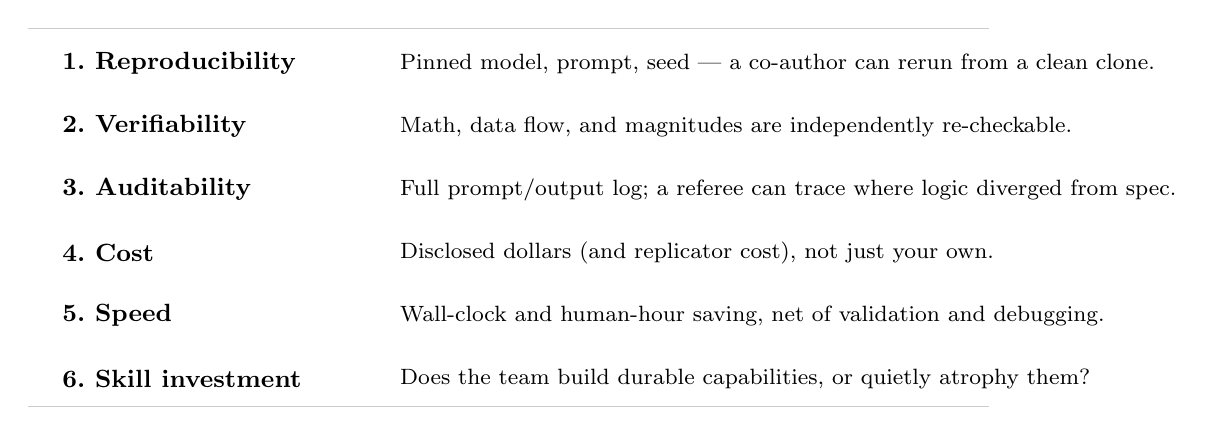
\begin{tikzpicture}
    \node[anchor=west, font=\small] at (0, 4.0) {$\square$ \textbf{1.\ Reproducibility}};
    \node[anchor=west, font=\footnotesize] at (4.4, 4.0) {Pinned model, prompt, seed --- a co-author can rerun from a clean clone.};

    \node[anchor=west, font=\small] at (0, 3.2) {$\square$ \textbf{2.\ Verifiability}};
    \node[anchor=west, font=\footnotesize] at (4.4, 3.2) {Math, data flow, and magnitudes are independently re-checkable.};

    \node[anchor=west, font=\small] at (0, 2.4) {$\square$ \textbf{3.\ Auditability}};
    \node[anchor=west, font=\footnotesize] at (4.4, 2.4) {Full prompt/output log; a referee can trace where logic diverged from spec.};

    \node[anchor=west, font=\small] at (0, 1.6) {$\square$ \textbf{4.\ Cost}};
    \node[anchor=west, font=\footnotesize] at (4.4, 1.6) {Disclosed dollars (and replicator cost), not just your own.};

    \node[anchor=west, font=\small] at (0, 0.8) {$\square$ \textbf{5.\ Speed}};
    \node[anchor=west, font=\footnotesize] at (4.4, 0.8) {Wall-clock and human-hour saving, net of validation and debugging.};

    \node[anchor=west, font=\small] at (0, 0.0) {$\square$ \textbf{6.\ Skill investment}};
    \node[anchor=west, font=\footnotesize] at (4.4, 0.0) {Does the team build durable capabilities, or quietly atrophy them?};

    \draw[gray!40] (-0.2, 4.45) -- (12, 4.45);
    \draw[gray!40] (-0.2, -0.35) -- (12, -0.35);
\end{tikzpicture}
\end{center}

\vspace{0.1cm}
\begin{center}
\textit{If any answer is ``no'' or ``I don't know,'' the artifact is not yet research-grade.}
\end{center}
\end{frame}

% ---- T6-F07 · EDIT · TIER: READ · from T6:156
% TODO(Phase B): Review A5: reframe as non-delegable responsibility (the researcher bears the residual claim), not "categorically outside the system"; compatible with HA-Ramsey's AI-surfaced discoveries.
\begin{frame}{Three Things AI Cannot Do --- Regardless of Capability}
\small
\begin{itemize}
  \item \textbf{Identification.} \\
  Choosing the variation that answers the causal question. \\
  An LLM does not know which shock is exogenous, which instrument is valid, or which event window is contaminated. It can describe identification strategies; it cannot \emph{certify} one for your setting.

  \vspace{0.1cm}
  \item \textbf{Welfare.} \\
  Choosing the objective function that defines ``good.'' \\
  Pareto weights, planner discount rates, equity--efficiency trade-offs --- these are normative choices the researcher must own.

  \vspace{0.1cm}
  \item \textbf{Judgment.} \\
  Choosing which question is worth asking. \\
  AI optimizes against a stated target; only economists decide which target is interesting, novel, and policy-relevant.
\end{itemize}

\vspace{0.15cm}
\begin{center}
\textit{These are not gaps that scale away with model size --- they are categorically outside the system.}
\end{center}
\end{frame}

% ---- T6-F08 · EDIT · TIER: READ · from T6:180
\begin{frame}{When NOT to Use an Agent}
\textbf{The six criteria can also serve as a boundary: there are research tasks where the agent overhead exceeds the benefit, or where the failure mode is too costly.}

\vspace{0.2cm}

\begin{itemize}
    \item \textbf{One-line scripts and isolated edits.} A two-line \texttt{sed} or one-shot plot has no validation surface for the harness to add value. Open the editor.
    \item \textbf{Deeply proprietary or undocumented pipelines.} If the conventions live in one person's head, the agent has nothing to read; the time you would spend documenting the pipeline well enough to brief the agent is the same time you would spend just fixing the thing.
    \item \textbf{Strict deterministic guarantees.} For numerical reproducibility audits, regulatory pipelines, or replication packages, model nondeterminism is a hazard the harness cannot fully suppress. Run it pinned; do not let the agent retry.
    \item \textbf{Restricted-data analyses where prompts may leak.} If pasting one column would violate IRB or HIPAA, the agent does not belong in the loop; the red-lines workarounds apply.
    \item \textbf{Tasks where you do not yet have a benchmark.} Without a way to validate, faster output just means faster wrong. Define the V0 benchmark first; \emph{then} bring in the agent.
\end{itemize}

\vspace{0.1cm}
\footnotesize\textbf{Practical rule:} the agent is most useful when the work is bounded, validated, and repeatable. None of those? Skip the agent.
\end{frame}

% ---- T6-F09 · KEEP · TIER: READ · from T6:197
\begin{frame}{Trust but Verify}
\begin{enumerate}
    \item Reproduce one statistic by hand
    \item Cross-check one result with another package or script
    \item Test a limiting case or zero-variance benchmark
    \item Read the code line by line where the economics enters
    \item Ask whether the magnitude and sign make sense
\end{enumerate}

\vspace{0.3cm}

\textbf{This is not optional ceremony.} It is what turns fast code into defensible research.
\end{frame}

% ---- T6-F10 · KEEP · TIER: READ · from T6:211
\begin{frame}{What Changes for Economic Research}
\begin{itemize}
    \item The distance from question to first result shrinks
    \item More specifications become cheap enough to try
    \item Reproducibility can improve because workflow is written down
    \item The premium shifts away from typing speed and toward design, judgment, and validation
\end{itemize}

\vspace{0.3cm}

\textbf{What stays human:} asking the question, choosing the design, knowing the data, and interpreting the output.
\end{frame}

% ---- T5-F20 · MOVE · TIER: READ · from T5:453
\begin{frame}{The Paradigm Shift, Completed: What Changed, What Did Not}
\textbf{The HA-Ramsey record, read one last time --- now as a statement about your role.}

\vspace{0.15cm}

\begin{columns}[T]
\begin{column}{0.49\textwidth}
\textbf{What changed}
\begin{itemize}
    \item Theory--code--debug loop compressed from months to days
    \item Documentation became executable: the TeX note, pseudocode, and code stay synchronized
    \item Cross-literature imports got cheap (computational geometry, viability theory)
    \item The unit of progress became the \emph{validated milestone}
\end{itemize}
\end{column}
\begin{column}{0.47\textwidth}
\begin{cautionbox}
\footnotesize
\textbf{What did NOT change:}
\begin{itemize}
    \item AI never decided what was economically interesting
    \item AI never caught the wrong timing on its own
    \item AI never knew when a result was not credible
\end{itemize}
\end{cautionbox}
\vspace{0.1cm}
\footnotesize\textit{``Weeks, not years --- and the binding constraint was economist judgment at the milestones, not implementation labor.''}
\end{column}
\end{columns}

\vspace{0.05cm}

\textbf{Read the two columns together:} the machine moved every bound except the one that defines the researcher.

{\scriptsize \textit{Source: HA-Ramsey case-study package (Lec10 T8).}}
\end{frame}


%=============================================================================
\section{Action Plan}
%===========================================================

\sectiondivider{Action Plan}{Your first thirty days}

% ---- NEW · TIER: CORE
% TODO(Phase B): Four-week strip: week 1 Git + instructions file + first session (T2b); week 2 first homotopy ladder with a benchmark (T5a); week 3 first agent from the canvas + detection matrix (T3a/T4); week 4 first scripted rung-3 run + audit + AI_LOG.md (T3b/T5c); mapped to capstone milestones M1/M2; harness-neutral.
\begin{frame}{Your First 30 Days}
\textbf{Placeholder --- written in Phase B.} The specification is in the source comment above this frame.
\end{frame}

% ---- NEW · TIER: READ
% TODO(Phase B): From archive v1:2417 -- the verbatim seven-line prompt (v1:2426-2435) with its rationale.
\begin{frame}{Your First Exercise: Clean Up Old Code}
\textbf{Placeholder --- written in Phase B.} The specification is in the source comment above this frame.
\end{frame}

% ---- T6-F12 · EDIT · TIER: READ · from T6:245
% TODO(Phase B): Keep the paraphrase; point to the verbatim prompt on the previous frame.
\begin{frame}{First Exercise and Looking Ahead}
\textbf{Best first exercise:} take one old project and ask an agent to help clean it up safely.

\vspace{0.25cm}

\begin{itemize}
    \item put the project under Git
    \item create a simple \texttt{CLAUDE.md}
    \item identify one repeated workflow worth encoding
    \item rerun the cleaned project and compare outputs
\end{itemize}

\vspace{0.3cm}

\textbf{Lec.~10:} we return to case studies and let students run a full workflow themselves.

\vspace{0.15cm}

\textit{If you want setup details for the lab, see the appendix.}
\end{frame}


%=============================================================================
\section{Next --- Lecture 10}
%===========================================================

\sectiondivider{Next --- Lecture 10}{From workflow logic to concrete case studies}

% ---- T6-F02 · MOVE · TIER: READ · from T6:45
% TODO(Phase B): Include Case 7 (Lec10 T9) among the patterns.
\begin{frame}{Lecture 10 Preview: Four Concrete Workflow Patterns}
\begin{center}
\small
\begin{tabular}{|p{2.7cm}|p{3.7cm}|p{4.7cm}|}
\hline
\textbf{Pattern} & \textbf{Lecture 10 case} & \textbf{What students will see} \\ \hline
Reusable skill & Paper-review workflow & staged quality control, quote checks, editorial filter \\ \hline
Empirical pipeline & MEPS uninsurance & harmonization, survey weights, benchmark validation, figures \\ \hline
Public-web dataset & Fellows metadata & source restrictions, provenance, missingness discipline \\ \hline
Full-lifecycle collaborator & Glue-work research project & theory, pipeline design, critique, claims discipline \\ \hline
\end{tabular}
\end{center}

\vspace{0.25cm}
\textbf{Why this matters:} Lec.~9 gives the workflow logic. Lec.~10 shows how the same logic changes shape across different research artifacts.
\end{frame}

% ---- T6-F03 · MOVE · TIER: READ · from T6:62
\begin{frame}{One Visual Hook from Lecture 10: MEPS Uninsurance}
\textbf{Case Study 2 asks:} who is uninsured in the United States, 2000--2023, and how did the ACA change the distribution?

\vspace{0.25cm}

\begin{center}
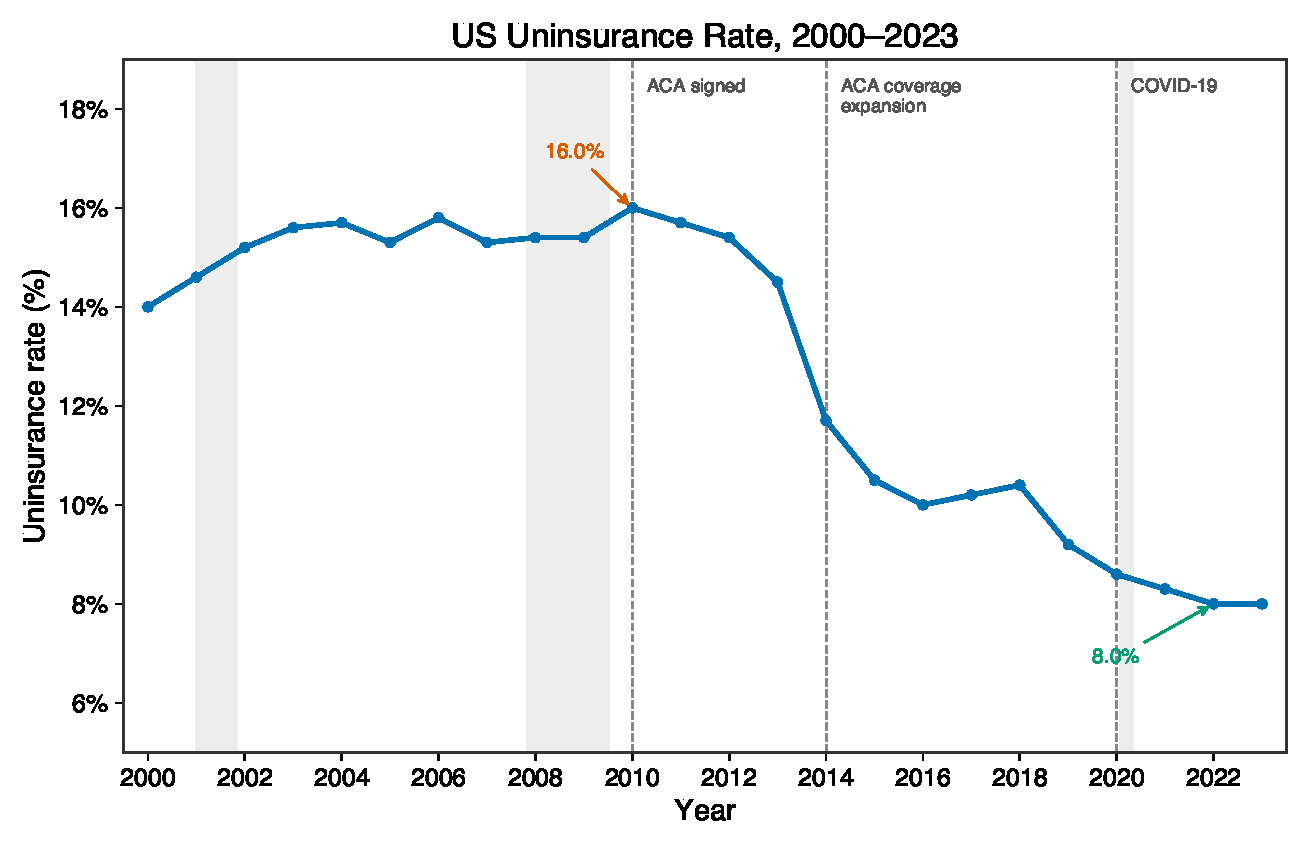
\includegraphics[height=0.38\textheight]{fig_overall_uninsurance.pdf}
\end{center}

\textbf{Why keep this figure here:} it is an accessible policy example for economists outside macro, and it shows what a validated empirical artifact looks like after the workflow succeeds.

\vspace{0.15cm}

\textbf{Lec.~10 adds the full pipeline:} prompts, schema harmonization, survey weights, external benchmarks, and subgroup figures.
\end{frame}

% ---- T6-F04 · EDIT · TIER: READ · from T6:78
% TODO(Phase B): Review A5: rewrite without IV vocabulary ("what role does the agent's output play in your inference?"), or cut.
\begin{frame}{Three Econometric Roles in Agent-Assisted Research}
\textbf{Lec07 T4 introduced a taxonomy: every text-derived variable plays one of three roles --- \emph{signal}, \emph{outcome}, or \emph{instrument}. The four Lec10 patterns get sharper when we apply that lens.}

\vspace{0.18cm}

\begin{center}
\footnotesize
\renewcommand{\arraystretch}{1.15}
\begin{tabular}{|p{2.7cm}|p{2.4cm}|p{2.6cm}|p{3.4cm}|}
\hline
\textbf{Pattern} & \textbf{Signal} & \textbf{Outcome} & \textbf{Instrument} \\ \hline
Reusable skill (paper review) & methodological rigor & review quality & staged evaluation rubric \\ \hline
Empirical pipeline (MEPS) & uninsurance rates & health-coverage estimates & survey-weighted harmonization \\ \hline
Public-web dataset (fellows) & field assignment & provenance log & source-restriction rules \\ \hline
Full-lifecycle collaborator (glue-work) & research idea & validated claims & agent $+$ domain expert critique \\ \hline
\end{tabular}
\end{center}

\vspace{0.12cm}
\textbf{Same agent toolkit, four research designs.} The taxonomy makes you ask: what role does the agent's output play in your inference?
\end{frame}

% ---- T6-F05 · MOVE · TIER: READ · from T6:100
\begin{frame}{What to Watch for in Lecture 10}
\begin{itemize}
    \item \textbf{Paper review:} how a reusable skill turns a vague prompt into a staged quality-control workflow
    \item \textbf{MEPS pipeline:} how an empirical question becomes a validated panel and figure set
    \item \textbf{Fellows dataset:} how provenance and missingness rules matter as much as code
    \item \textbf{Glue-work project:} how agentic AI can act as a full-lifecycle collaborator without replacing human claims discipline
\end{itemize}

\vspace{0.3cm}
\textbf{Bridge from Lec.~9 to Lec.~10:} today's lecture explains the logic of the workflow; next lecture shows the artifacts it can produce.
\end{frame}

% ---- T5-F21 · EDIT · TIER: CORE · from T5:490
% TODO(Phase B): The all-complete map is the finale (review A9); fold in T6-F11's epigraph ("Agents can lay bricks quickly. You still design the structure.") in the takeaway.
% TODO(Phase B): Rewrite the three-question sentence to match the map's bands: how it works (9.1-9.2), how to build and use it (9.3-9.4), your role (9.5, where the homotopy method and the managed project now live).
\begin{frame}{Your Job Description: PI and Project Manager}
\textbf{The three questions, answered:} \emph{how it works} --- a tool-calling loop steered by files (Parts 9.1--9.2); \emph{how to use it well} --- the homotopy method inside a managed project (Parts 9.3--9.5); \emph{your role} --- this frame.

\LecNineMap{0}{}

\begin{takeawaybox}
\footnotesize
\textbf{Set the goal. Define the final product. Gate every intermediate good. Assign the work --- sessions, agents, sub-agents. Cross-verify everything. And remain the client of the outside view:} the one thing your agent cannot give you is a prior other than your own.
\end{takeawaybox}
\end{frame}

% ---- NEW · TIER: CORE
% TODO(Phase B): v1 bridge + T5-F22's hand-off bullets: "Lecture 9 explained the logic; Lecture 10 shows the artifacts. You saw the fellows workflow --- Lec10 T4 shows the findings and Exercise B gives you your own batch; you saw HA-Ramsey's contract and milestones --- Lec10 T8 shows the discoveries."
% TODO(Phase B): Close on Lec10 T9: "the agent didn't break the rules --- it followed them; the loophole was in the contract" (review A3).
\begin{frame}{Bridge: Lecture 10 Shows the Artifacts}
\textbf{Placeholder --- written in Phase B.} The specification is in the source comment above this frame.
\end{frame}

%===========================================================
\end{document}
